\documentclass[11pt,a4paper]{article}
\usepackage[utf8]{inputenc}
\usepackage{a4wide}
\usepackage{fancyhdr}
\pagestyle{fancy}
\thispagestyle{fancy}

\usepackage{gensymb}
\usepackage{hyperref}
\newcommand\fnurl[2]{%
  \href{#2}{#1}\footnote{\url{#2}}%
}
\usepackage{amsfonts}
% Bibliografía
\usepackage{natbib}

\usepackage[spanish]{babel}
\parskip = 11pt
\addtolength{\topmargin}{-1cm}
\addtolength{\textheight}{2.2cm}
\addtolength{\textwidth}{-.5cm}

\makeatletter
\renewcommand\paragraph{\@startsection{paragraph}{4}{\z@}%
            {-2.5ex\@plus -1ex \@minus -.25ex}%
            {1.25ex \@plus .25ex}%
            {\normalfont\normalsize\bfseries}}
\makeatother
\setcounter{secnumdepth}{4} % how many sectioning levels to assign numbers to
\setcounter{tocdepth}{4}    % how many sectioning levels to show in ToC

\usepackage[conEntregas]{caratula}
\materia{Teoría de las Comunicaciones}
\titulo{Trabajo Práctico I}
\subtitulo{\textit{Wiretapping}}
\integrante{Fernández, Gonzalo}{836/10}{gpfernandezflorio@gmail.com}
\integrante{Aleman, Damián Eliel}{377/10}{damianealeman@gmail.com}
\integrante{Pizzagalli, Matías}{257/12}{matipizza@gmail.com}

\begin{document}

\maketitle

\tableofcontents

\newpage


\section{Introducción Te\'orica}

%Este trabajo consistió en realizar una lectura de paquetes de diversas redes realizada por una herramienta implementada en $python$ utilizando \texttt{scapy} para acceder a la placa de red. Luego de realizar la herramienta analizamos los paquetes 
Supongamos que tenemos una fuente que emite una secuencia de símbolos pertenecientes a un alfabeto finito y determinado $S = \{s_1, s_2, .., s_q\}$. Los símbolos emitidos sucesivamente se eligen de acuerdo con una ley fija de probabilidad. Si los símbolos emitidos son estadísticamente independientes, se dice que la fuente $S$ es \textbf{de memoria nula}.

Si consideramos la \textbf{información} suministrada por una fuente de memoria nula, la cantidad \emph{media} de información por símbolo está dado por la fórmula:
\begin{center}
    $\displaystyle \sum_S P(s_i) I(s_i)$ bits
\end{center}


Definimos entonces a la \textbf{entropía} como la \textbf{cantidad media de información por símbolo de una fuente de memoria nula}. La notamos $H(S)$
\begin{center}
$\displaystyle H(S) = \sum_S P(s_i)\ log(\frac{1}{P(s_i)})$ bits
\end{center}

Luego se puede ver a la fuente S que tiene como símbolos a los protocolos utilizados en la red en un intervalo de tiempo dado.
Por otro lado podemos pensar a un símbolo como distinguido cuando sobresale del resto en términos de la información que provee.
En el siguiente trabajo analizaremos distintas redes basándonos en la entropía como métrica, 
para poder diferenciar a los protocolos y a los nodos distinguidos de las respectivas redes.

Cabe destacar que el análisis para distinguir los nodos en las redes lo haremos solamente sobre el protocolo $ARP$.
$ARP$ (del inglés Adress Resolution Protocol) es un protocolo de comunicaciones de la capa de enlace de datos, responsable de encontrar la dirección de hardware (Ethernet MAC) que corresponde a una determinada dirección IP. Para ello se envía un paquete (ARP request) a la dirección de difusión de la red (broadcast, MAC = FF:FF:FF:FF:FF:FF) que contiene la dirección IP por la que se pregunta, y se espera a que esa máquina (u otra) responda (ARP reply) con la dirección Ethernet que le corresponde. Cada máquina mantiene una caché con las direcciones traducidas para reducir el retardo y la carga. ARP permite a la dirección de Internet ser independiente de la dirección Ethernet, pero esto solo funciona si todas las máquinas lo soportan.
 \footnote{ARP está documentado en el RFC 826 \url{https://tools.ietf.org/html/rfc826}}


\section{Desarrollo}

Para la implementación de las consignas pedidas se utilizó el lenguaje de programación \texttt{python}, tal como
fue recomendado por la cátedra. Para acceder a la placa de red se utilizó el paquete \texttt{scapy} que provee
funciones específicas para ello.

\subsection{Implementación (Primera consigna: capturando tráfico)}

\subsubsection{Ejercicio 1}
El código que implementa la herramienta que escucha pasivamente los paquetes Ethernet de la red es \texttt{e1.py}
y se encuentra en el directorio \texttt{src}. Toma como parámetro opcional un entero que se traduce en la cantidad
de segundos que va a permanecer activo. El valor por defecto es $10$ segundos. La función \texttt{main} del script
utiliza la función \texttt{sniff} del paquete \texttt{scapy} pasándole como parámetro de \texttt{timeout} el
parámetro ingresado (o $10$ si no se ingresó ninguno) y como parámetro de \texttt{prn} la función
\texttt{monitor\_callback} que toma un paquete de red y lo imprime mediante un llamado a la función \texttt{show}.
La forma de ejecutarlo es

\[
\texttt{\$ sudo python e1.py [TIMEOUT]}
\]

Notar que para ejecutarlo se necesitan permisos de administrador ya que la función \texttt{sniff} de \texttt{scapy}
necesita permisos para acceder a la placa de red.

\subsubsection{Ejercicio 2}
El código que implementa la herramienta para calcular la entropía de la fuente S en la red local es \texttt{e2.py}
y se encuentra en el directorio \texttt{src}. Este programa es una modificación del anterior, \texttt{e1.py}.
La principal modificación es que los paquetes obtenidos por el llamado a \texttt{sniff} ahora se almacenan para
operar sobre ellos luego. Se anula el parámetro \texttt{prn} pero se conserva el \texttt{timeout} (el cuál sigue
siendo un parámetro opcional del programa). Una vez recibidos todos los paquetes, se obtiene el tipo de cada uno
mediante el atributo \texttt{type}. En este punto encontramos que no todos los paquetes capturados poseen dicho
atributo, así que atrapamos una excepción al leer el tipo. En caso de saltar la excepción, consideramos que el
paquete tiene tipo $0x0000$ y lo imprimimos llamando a \texttt{monitor\_callback}. A través de la función de
mapeo \texttt{map\_number\_to\_name} convertimos a una cadena el valor del tipo del paquete. Esta función
utiliza un diccionario basado en la siguiente tabla\footnote{https://en.wikipedia.org/wiki/EtherType}:

\begin{tabular}{|r|l|c|r|l|c|r|l|}
\hline
0x0800 & IPv4 & & 0x8847 & MPLS Unicast & & 0x88CD & SERCOS III \\
\hline
0x0806 & ARP & & 0x8848 & MPLS Multicast & & 0x88E1 & HomePlug AV \\
\hline
0x0842 & WakeOn LAN & & 0x8863 & PPPoE Discovery & & 0x88E3 & MRP \\
\hline
0x22F3 & IETF TRILL & & 0x8864 & PPPoE Session & & 0x88E5 & MAC security \\
\hline
0x6003 & DECnet & & 0x8870 & Jumbo & & 0x88E7 & PBB \\
\hline
0x8035 & RARP & & 0x887B & HomePlug 1.0 & & 0x88F7 & PTP \\
\hline
0x809B & Ethertalk & & 0x888E & 802.1X & & 0x8902 & CFM \\
\hline
0x80F3 & AARP & & 0x8892 & PROFINET & & 0x8906 & FCoE \\
\hline
0x8100 & 802.1Q & & 0x889A & SCSI & & 0x8914 & FCoE Init \\
\hline
0x8137 & IPX & & 0x88A2 & ATA & & 0x8915 & RoCE \\
\hline
0x8204 & QNX Qnet & & 0x88A4 & EtherCAT & & 0x891D & TTE  \\
\hline
0x86DD & IPv6 & & 0x88A8 & 802.1ad & & 0x892F & HSR \\
\hline
0x8808 & EFC & & 0x88AB & Powerlink & & 0x9000 & ECTP \\
\hline
0x8819 & CobraNet & & 0x88CC & LLDP & & & \\
\hline
\end{tabular}

Luego se utiliza la función \texttt{Counter} de \texttt{python} para generar el diccionario \texttt{cantidades}
cuyas claves son los tipos de protocolos y sus respectivos valores son la cantidad de paquetes de tal tipo.
A partir de este diccionario (el cual se imprime para verificación) se calcula la probabilidad de cada tipo.
Finalmente se calcula la entropía de la fuente utilizando la probabilidad de cada tipo y se la imprime. La
forma de ejecutarlo es:

\[
\texttt{\$ sudo python e2.py [TIMEOUT]}
\]

\subsubsection{Ejercicio 3}
Para poder distinguir los nodos de un red, se nos ocurrio proponer como posibles fuentes de información la IP destino y la IP origen de los paquetes ARP. Nos parece interesante medir ambas fuentes de información propuestas para luego poder analizarlas y llegar a distinguir cuales son los nodos que mas envian y mas reciben paquetes y de esta forma comprender la topologia de la red en cuestion.

Implementar este programa consistió en modificar el anterior, ya que la única diferencia entre ambas
consignas es el atributo de cada paquete utilizado como símbolo de la fuente. Al llamado a la función \texttt{sniff}
se le agregó el parámetro \texttt{filter=``arp''} para que sólo se examinen los paquetes \texttt{ARP}. Luego, en lugar de
obtener el tipo de cada paquete, que ya sabemos que todos son ARP, lo que se obtiene es la IP origen y la IP destino de cada paquete.
El resto del código es idéntico al de \texttt{e2.py}. La forma de ejecutarlo es:

El código que implementa la herramienta de distinción de nodos (hosts) de la red, basada únicamente en paquetes que
utilizan el protocolo ARP es \texttt{e3.py} y se encuentra en el directorio \texttt{src}.

\[
\texttt{\$ sudo python e3.py [TIMEOUT]}
\]

\subsection{Experimentación (Segunda consigna: gráficos y análisis)}

Para la parte de experimentación se implementó otro script de python que realiza una medición y sobre
esa medición calcula la entropía para las tres fuentes. De esta forma se pueden comparar los análisis
realizados sobre una misma muestra, cosa que no habríamos podido si ejecutábamos primero un script y luego
el otro. El programa correspondiente es \texttt{sniffer.py} y se encuentra en el directorio \texttt{src}.

La mayor parte del código es idéntica a la de \texttt{e2.py} y \texttt{e3.py} combinados. Sin embargo,
también se aplicaron algunas optimizaciones. Por ejemplo, ya no se almacenan los paquetes capturados por
\texttt{sniff}, sino que se procesan a medida que se capturan. Para ello, se modificó la función
\texttt{monitor\_callback} de forma que obtenga el tipo (tal como se hizo en \texttt{e2.py}) y, en caso
de ser un paquete \texttt{ARP}, la IP origen y la IP destino
(tal como se hizo en \texttt{e3.py}) de cada paquete a medida que son capturados. Es por esto que se volvió
a la versión original de \texttt{sniff} pasándole como parámetro \texttt{prn=monitor\_callback}. Tras finalizar
la escucha, se generan los diccionarios, se imprimen y se calculan las entropías. Además, se escribe a un archivo
los valores de cada diccionario para poder ser graficados como histogramas con \texttt{gnuplot}. La forma de
ejecutarlo es:

\[
\texttt{\$ sudo python sniffer.py FILE\_PREFIX [TIMEOUT]}
\]

El parámetro de \texttt{timeout} sigue siendo opcional (10 segundos por defecto). Los archivos de salida
se componen del prefijo \texttt{FILE\_PREFIX} pasado como parámetro obligatorio y las cadenas \texttt{Protocolos},
\texttt{IpsSrcArp} o \texttt{IpsDstArp}, según corresponda. Estos archivos se guardan en la carpeta \texttt{mediciones}.

%TODO: hipótesis: ipv4 > ipv6, #ARP en función del tamaño de la red, el router maneja mucho más paquetes que el resto de los nodos, etc.

\subsubsection{Experimento 1: Red hogareña}
\paragraph{Medición cableada de 10 minutos}

Este experimento consiste en ... %TODO

\paragraph{Medición inalámbrica de 10 minutos}

Este experimento consiste en ... %TODO

\subsubsection{Experimento 2: Red pública}
\paragraph{Medición inalámbrica de 10 minutos}

Este experimento consiste en ... %TODO

\paragraph{Medición inalámbrica de 60 minutos}

Este experimento consistie en ...%TODO

\subsubsection{Experimento 3: Red laboral}
\paragraph{Medición inalámbrica de 60 minutos}

Este experimento consistió en dos mediciones de una hora dos días distintos sobre una misma red.


\section{Resultados}

En la carpeta \texttt{mediciones} se encuentran los archivos de salida correspondientes a cada
experimento. Por cada uno, se adjunta un archivo \texttt{README.txt} con la información conocida
sobre la red en cuestión y otro arhivo \texttt{exceptions.txt} que describe los paquetes sin tipo
capturados. Los nombres de los experimentos denotan el tipo de red, el tipo de conexión y la
duración del experimento en minutos.

% \subsection{Experimento 1: Red hogareña, cableada, 10 mintos}
\subsection{Experimento 1: Red hogareña}
\subsubsection{Medición cableada}

\begin{center}
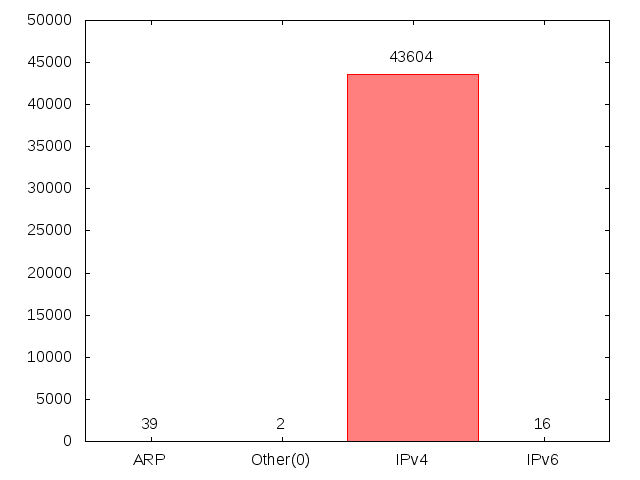
\includegraphics[width=8cm]{../mediciones/home-eth-10/home-eth-10Protocolos.png}
\end{center}

En este gráfico podemos observar que ARP se usa muy poco en relación con IP. Imaginamos que es porque hay pocos nodos en la red y se aprende rápido la configuración de la red.
En cuanto a la diferencia entre los distintas versiones de IP, nuestra hipótesis es que en general vamos a encontrar más paquetes IPv4 que IPv6 ya que todavía no se migró a la versión 6 del protocolo IP.
Dicha hipótesis se ve confirmada en este gráfico ya que la relación entre ambas versiones del protocolo es aproximadamente 2725 a 1 a favor de la versión 4.
Es claro que el tipo $0x0800$ correspondiente al protocolo IPv4, es un símbolo distinguido de la fuente \textbf{S} ya que es el que más aparece,
es decir que es el que tiene mayor probabilidad. El resto de los símbolos tienen frecuencias similares y mucho menores a la de $0x0800$.

\begin{minipage}{8cm}
  \centering
  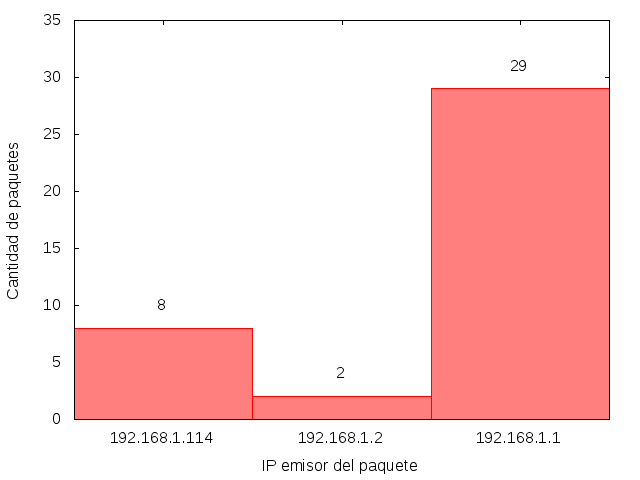
\includegraphics[width=8cm]{../mediciones/home-eth-10/home-eth-10IpsSrcArp.png}
\end{minipage}%
\begin{minipage}{8cm}
  \centering
  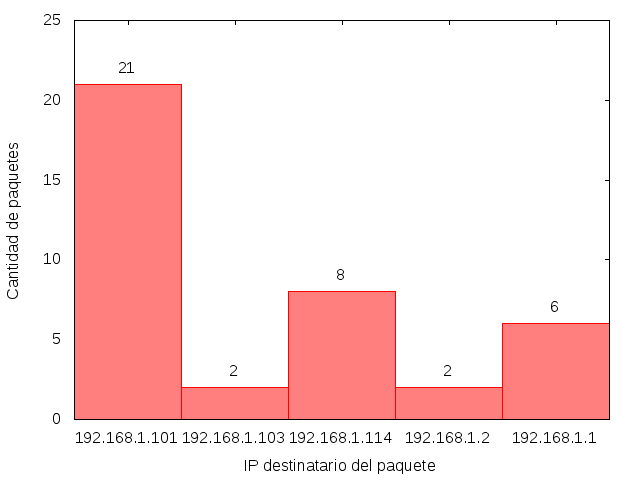
\includegraphics[width=8cm]{../mediciones/home-eth-10/home-eth-10IpsDstArp.png}
\end{minipage}

Vemos que para este experimento no tiene sentido considerar la IP del emisor de un paquete para identificar a los nodos de la red ya que sólo tres direcciones
(la de la computadora que está ejecutando el experimento y las de los dos routers) son visibles. Esto tiene sentido al considerar que la computadora que
está ejecutando el experimento está conectada al router principal (con dirección \textbf{192.168.1.1}) a través de un cable ethernet, por lo que los paquetes emitidos
por otros hosts no deberían llegar hasta este equipo. En cuanto a los destinatarios de los paquetes, vemos que el router no representa un símbolo distinguido
como sí lo hacía en la fuente de basada en emisores.

\begin{center}
\begin{tabular}{|c||c|}
\hline
Entropía de los protocolos & 0.0157726691884  \\
\hline
Entropía de las IPs origen de ARP & 1.00639070966  \\
\hline
Entropía de las IPs destino de ARP & 1.80467296546 \\
\hline
\end{tabular}
\end{center}

\subsubsection{Medición inalámbrica}

\begin{center}
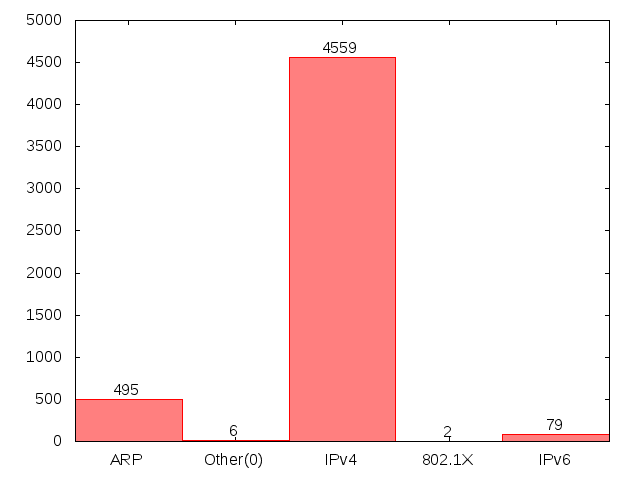
\includegraphics[width=8cm]{../mediciones/home-wfi-10/home-wfi-10Protocolos.png}
\end{center}

Otra vez se ve la superioridad de la versión 4 del protocolo IP, no sólo sobre la versión 6 del mismo protocolo, sino sobre el resto de los protocolos.
Sin embargo, la proporción es mucho menor. Al comparar este gráfico con el del experimento anterior, notamos dos cambios significativos. Por un lado la cantidad
de paquetes de tipo IPv4 es casi 10 veces menor. Por otro lado la cantidad de paquetes de tipo ARP y de tipo IPv6 se multiplicaron varias veces. Si consideramos
que la duración fue de 10 minutos para ambos experimentos, llama la atención esta diferencia. Como se puede ver en la siguiente tabla, los paquetes Ipv4 pasaron
de ocupar el 99.9\% de los paquetes capturados a ocupar el 88.7\%. Los de tipo IPv6 pasaron del 0.04\% al 1.54\% y los de tipo ARP pasaron del 0.09\% al 9.63\%.

\begin{center}
\begin{tabular}{|c||c|c|}
\hline
Protocolo & Red cableada & Red Wifi \\
\hline
ARP & 0.09\% & 9.63\% \\
\hline
IPv4 & 99.87\% & 88.68\% \\
\hline
IPv6 & 0.04\% & 1.54\% \\
\hline
Otros & 0.01\% & 0.16\% \\
\hline
\end{tabular}
\end{center}


\begin{minipage}{8cm}
  \centering
  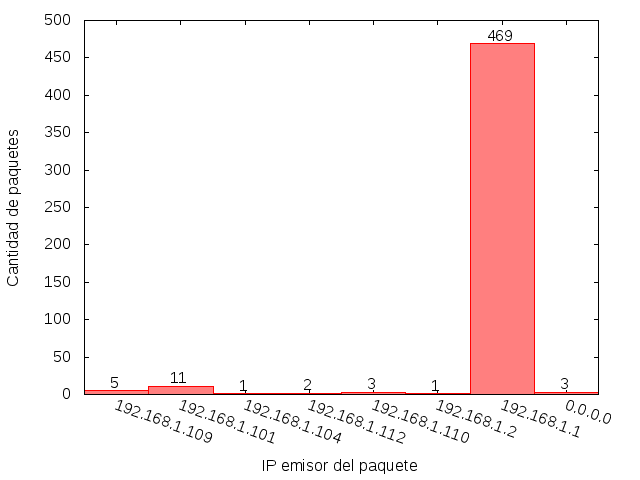
\includegraphics[width=8cm]{../mediciones/home-wfi-10/home-wfi-10IpsSrcArp.png}
\end{minipage}%
\begin{minipage}{8cm}
  \centering
  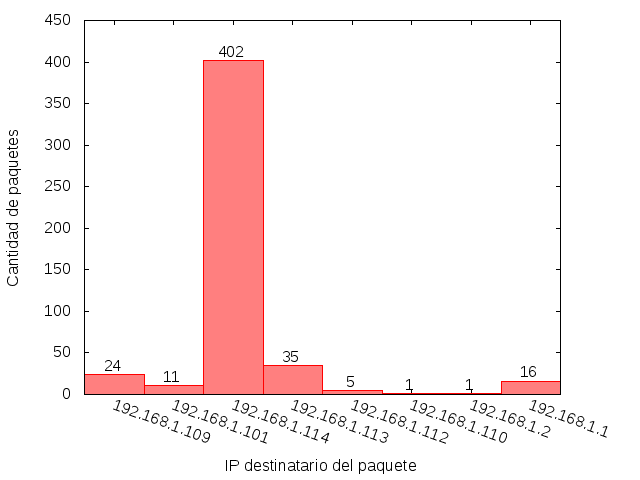
\includegraphics[width=8cm]{../mediciones/home-wfi-10/home-wfi-10IpsDstArp.png}
\end{minipage}


En cada uno de estos gráficos encontramos un nodo distinguido. Del lado de los emisores, la dirección IP distinguida corresponde al
router principal de la red, mientras que el nodo al que más paquetes van dirigidos es el host que ejecuta el experimento. El resto
de las direcciones mantiene una baja frecuencia de envío y recepción de paquetes. Otro punto a notar es la aparición de la dirección
\textbf{0.0.0.0} como emisor de 3 paquetes.

\begin{center}
\begin{tabular}{|c||c|}
\hline
Entropía de los protocolos & 0.5871665762  \\
\hline
Entropía de las IPs origen de ARP & 0.420338347182  \\
\hline
Entropía de las IPs destino de ARP & 1.11098133367 \\
\hline
\end{tabular}
\end{center}


\subsection{Experimento 2: Red pública}


\begin{minipage}{8cm}
  \centering
  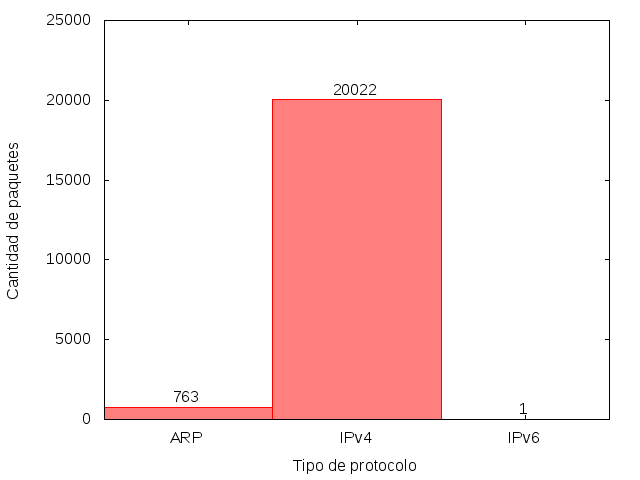
\includegraphics[width=8cm]{../mediciones/altop-wifi-10/altop10Protocolos.png}
  10 minutos
\end{minipage}%
\begin{minipage}{8cm}
  \centering
  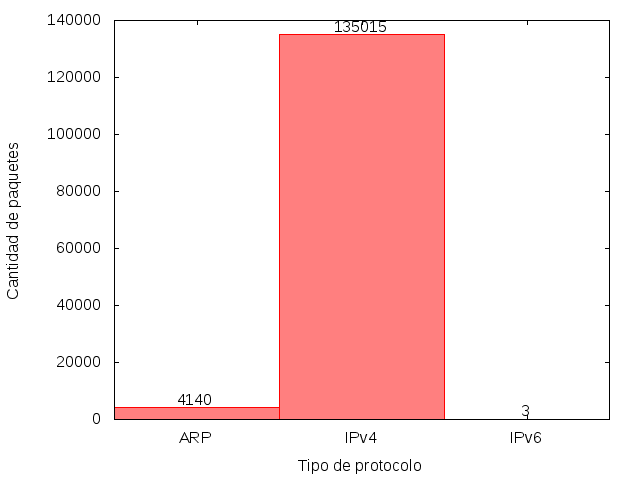
\includegraphics[width=8cm]{../mediciones/altop-wifi-60/altop60Protocolos.png}
  60 minutos
\end{minipage}


Seguimos viendo en esta red que el protocolo IPv4 es el más utilizado para el envío de paquetes. Es particularmente notoria la escasa
cantidad de paquetes de tipo IPv6, mucho menor que en la red hogareña del experimento anterior. Sí se incrementa la cantidad de paquetes
de tipo ARP en la misma cantidad de tiempo, respecto a la red hogareña. Esto puede deberse a que la red pública es considerablemente mayor.


\begin{minipage}{8cm}
  \centering
  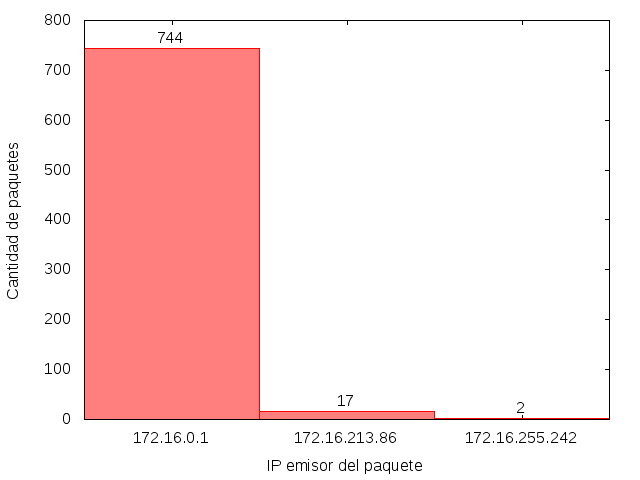
\includegraphics[width=8cm]{../mediciones/altop-wifi-10/altop10IpsSrcArp.png}
  10 minutos
\end{minipage}%
\begin{minipage}{8cm}
  \centering
  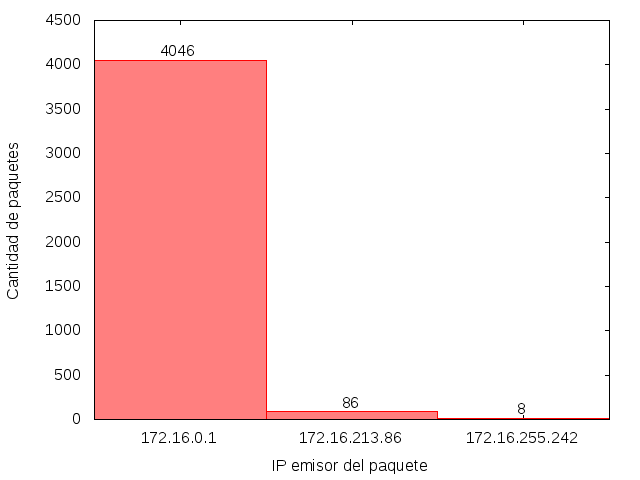
\includegraphics[width=8cm]{../mediciones/altop-wifi-60/altop60IpsSrcArp.png}
  60 minutos
\end{minipage}


En este caso nos encontramos con un comportamiento inesperado. Más del 97\% de los paquetes capturados fueron emitidos por una misma dirección
IP, que podemos suponer que es el router. Por otro lado, sólo pudieron identificarse 3 direcciones IP distintas en la red, a diferencia de lo
que había sucedido en la red hogareña, en la que se pudieron identificar varios nodos más. Claramente, la IP \textbf{172.16.0.1} es un símbolo
distinguido de la fuente.

\begin{center}
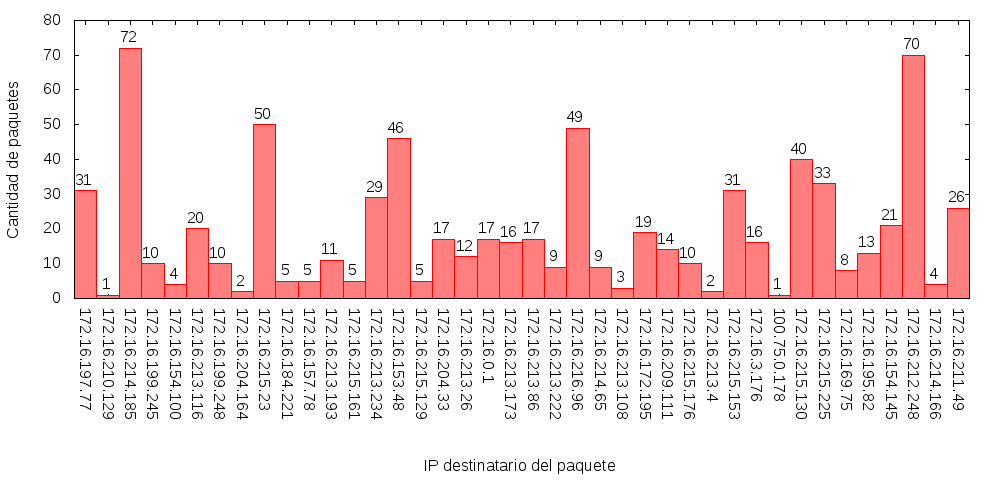
\includegraphics[width=16cm]{../mediciones/altop-wifi-10/altop10IpsDstArp.png}
10 minutos
\end{center}

\begin{center}
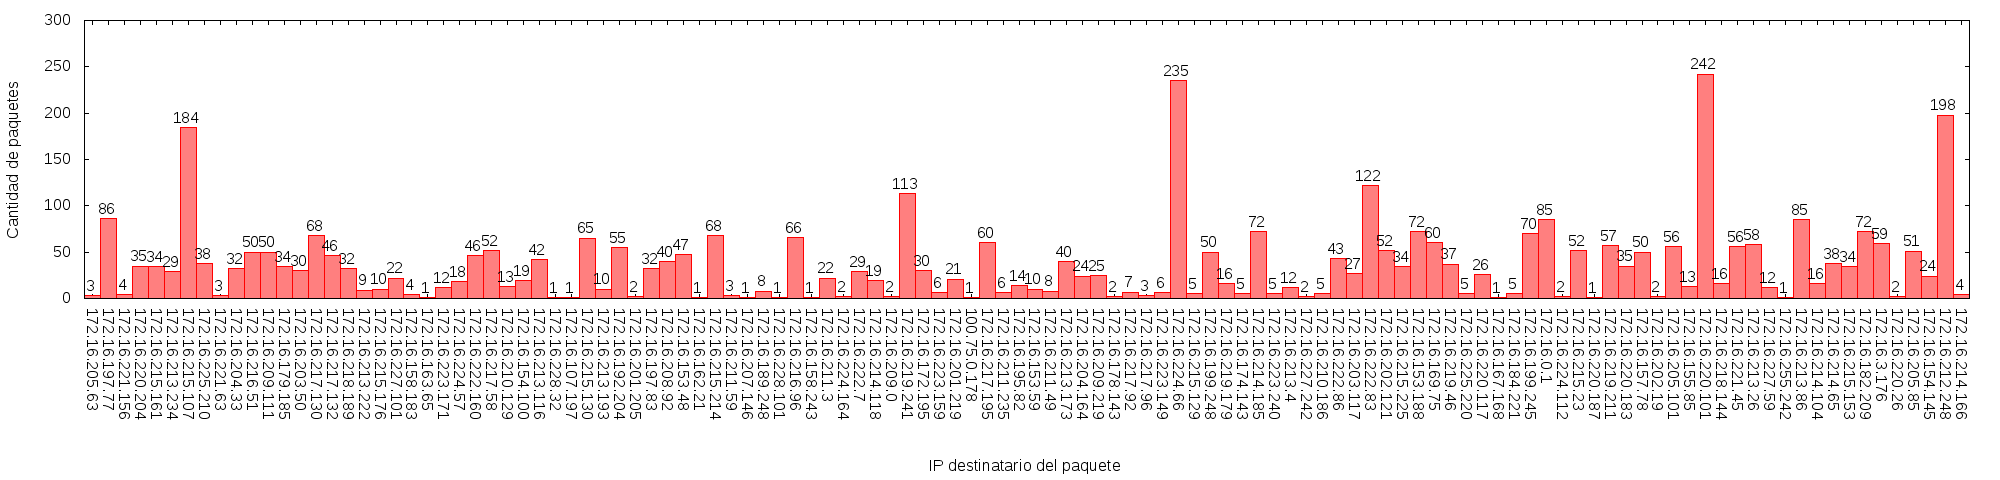
\includegraphics[width=16cm]{../mediciones/altop-wifi-60/altop60IpsDstArp.png}
60 minutos
\end{center}

Estos gráficos muestra algo más parecido a lo esperado en cuanto a la cantidad de nodos identificados. Lo que es incierto es la razón por la cual
los paquetes son dirigidos a tantos nodos distintos pero emitidos por un grupo reducido.
Para poder observar el segundo gráfico mejor, lo agregamos en el Apéndice, en la sección \ref{exp2_60_big}.

\begin{center}
\begin{tabular}{|c||c|c|}
\hline
 & 10 minutos & 60 minutos \\
\hline
\hline
Entropía de los protocolos & 0.227743354201 & 0.193502700102 \\
\hline
Entropía de las IPs origen de ARP & 0.180229910313 & 0.1659063338 \\
\hline
Entropía de las IPs destino de ARP & 4.77276412705 & 6.07060528117 \\
\hline
\end{tabular}
\end{center}

\subsection{Experimento 3: Red laboral}


\begin{minipage}{8cm}
  \centering
  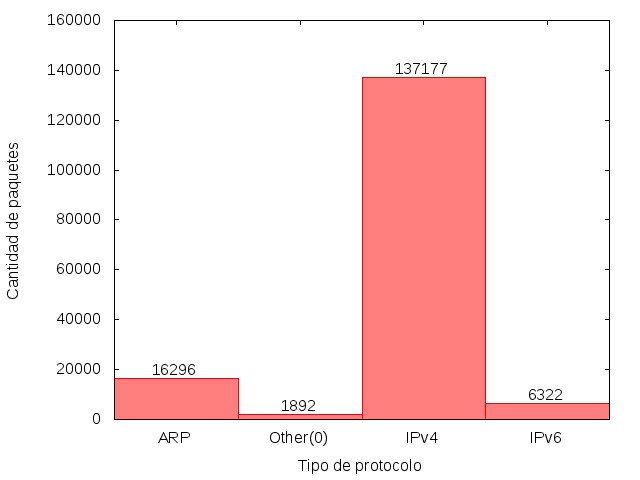
\includegraphics[width=8cm]{../mediciones/job1/type.png}
  Primera medición
\end{minipage}%
\begin{minipage}{8cm}
  \centering
  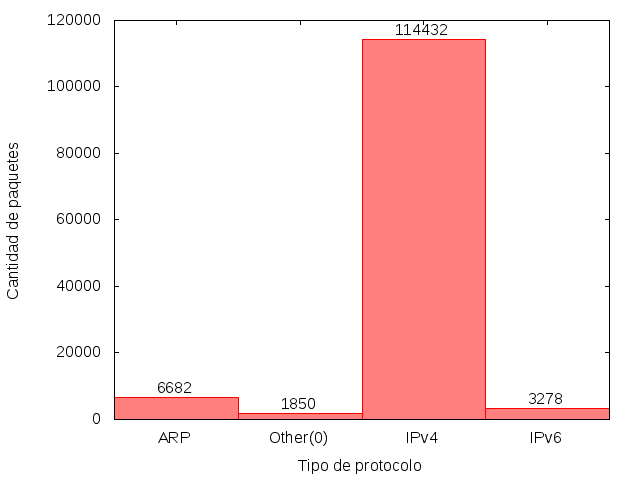
\includegraphics[width=8cm]{../mediciones/job2/type.png}
  Segunda medición
\end{minipage}


\begin{center}
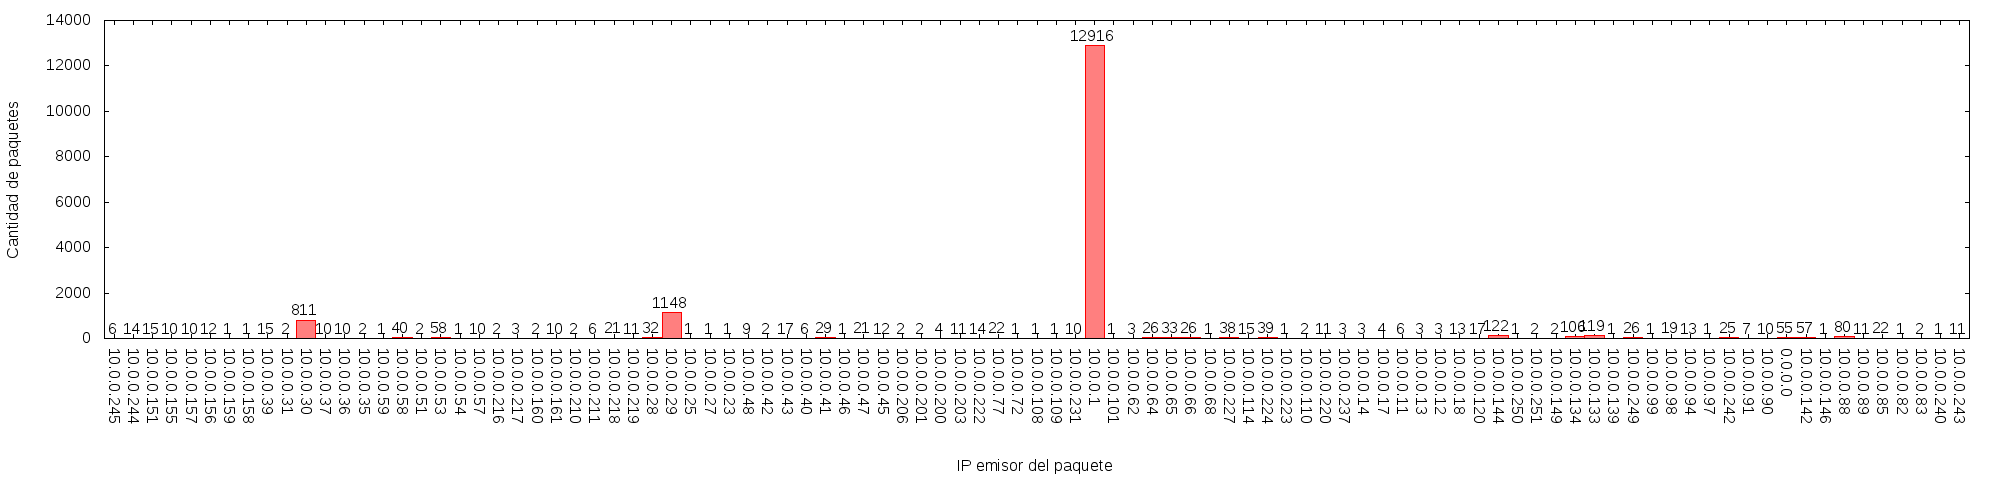
\includegraphics[width=16cm]{../mediciones/job1/src.png}
Primera medición
\end{center}

\begin{center}
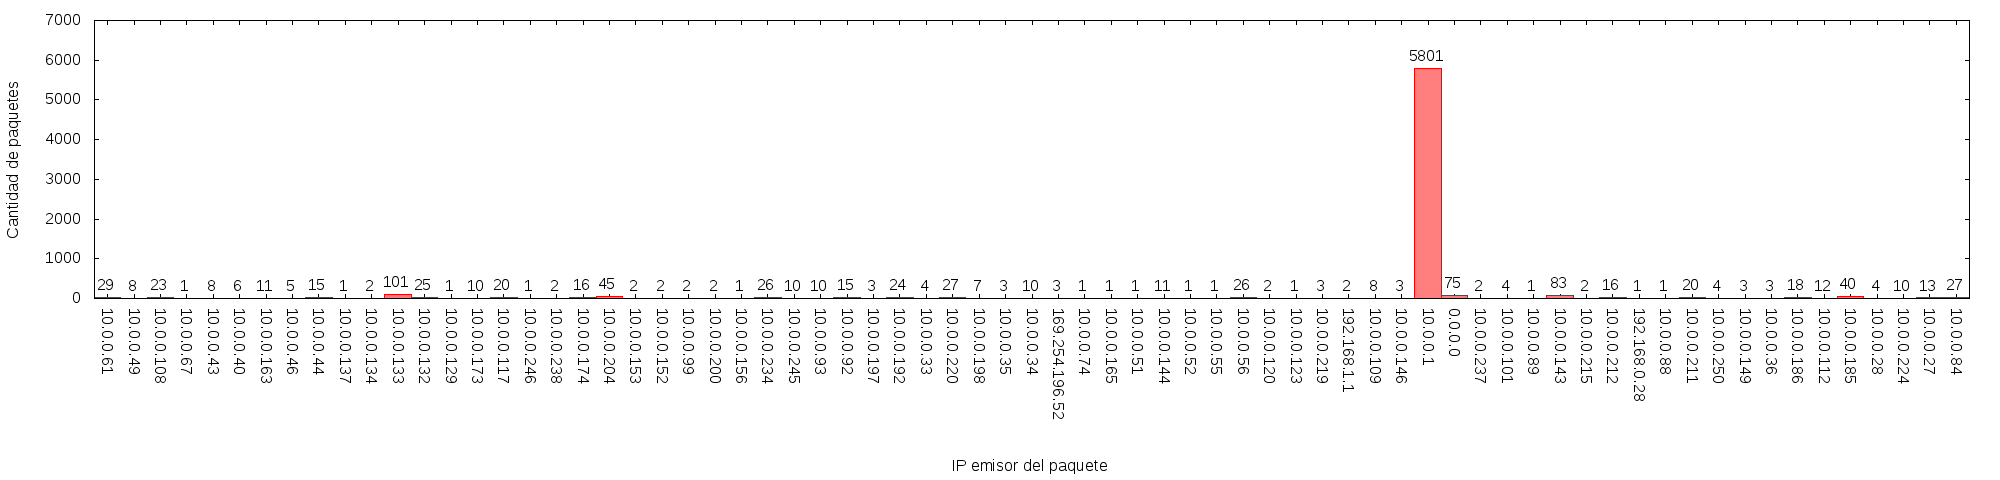
\includegraphics[width=16cm]{../mediciones/job2/src.png}
Segunda medición
\end{center}

A diferencia de lo que ocurría con la red pública del segundo experimento, en la que aparecían muchos nodos receptores pero pocos emisores,
en esta red podemos identificar una enorme cantidad de nodos a partir de las direcciones fuente de los paquetes ARP.
Nuevamente, identificamos un nodo (en este caso, con la dirección \textbf{10.0.0.1}) que envía casi la totalidad de los paquetes.
A pesar de que ambas mediciones son de una hora, la actividad es mucho mayor en la primera medición que en la segunda. Esto puede
deberse al horario en que fue realizado cada experimento.

\begin{center}
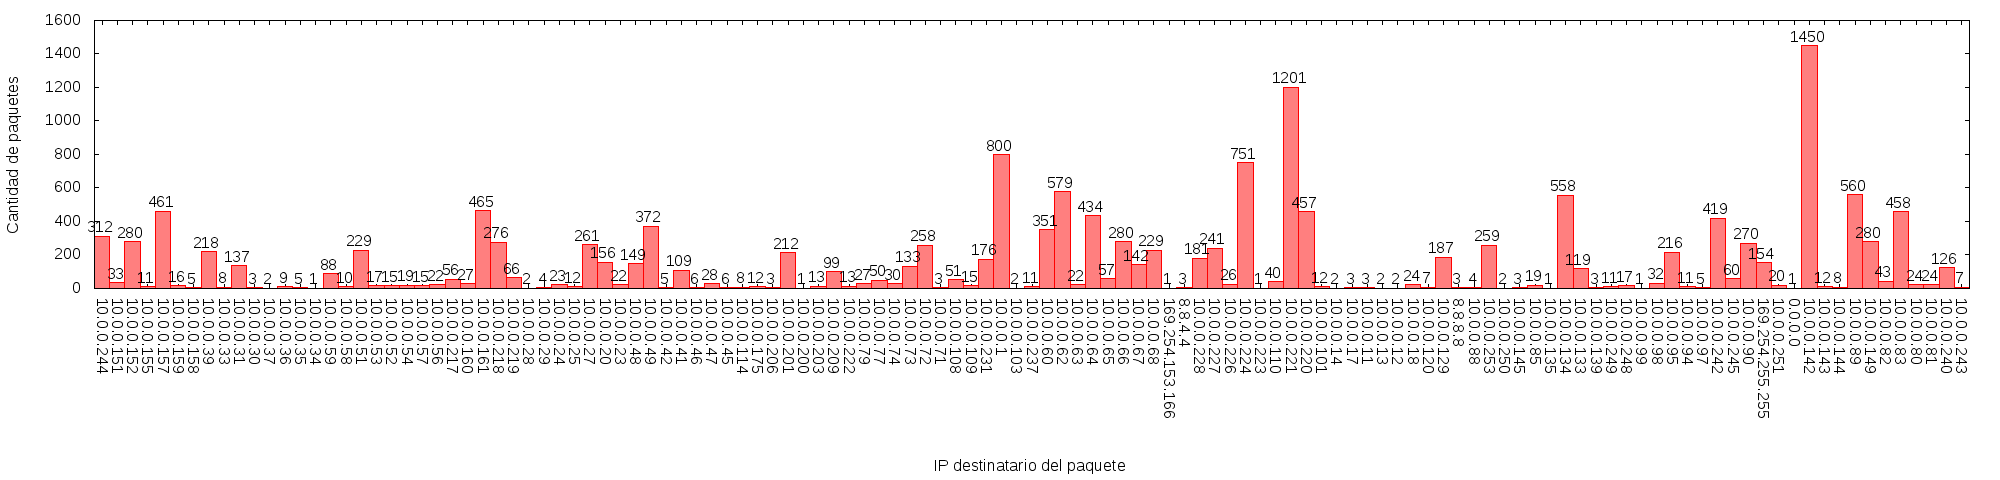
\includegraphics[width=16cm]{../mediciones/job1/dst.png}
Primera medición
\end{center}

\begin{center}
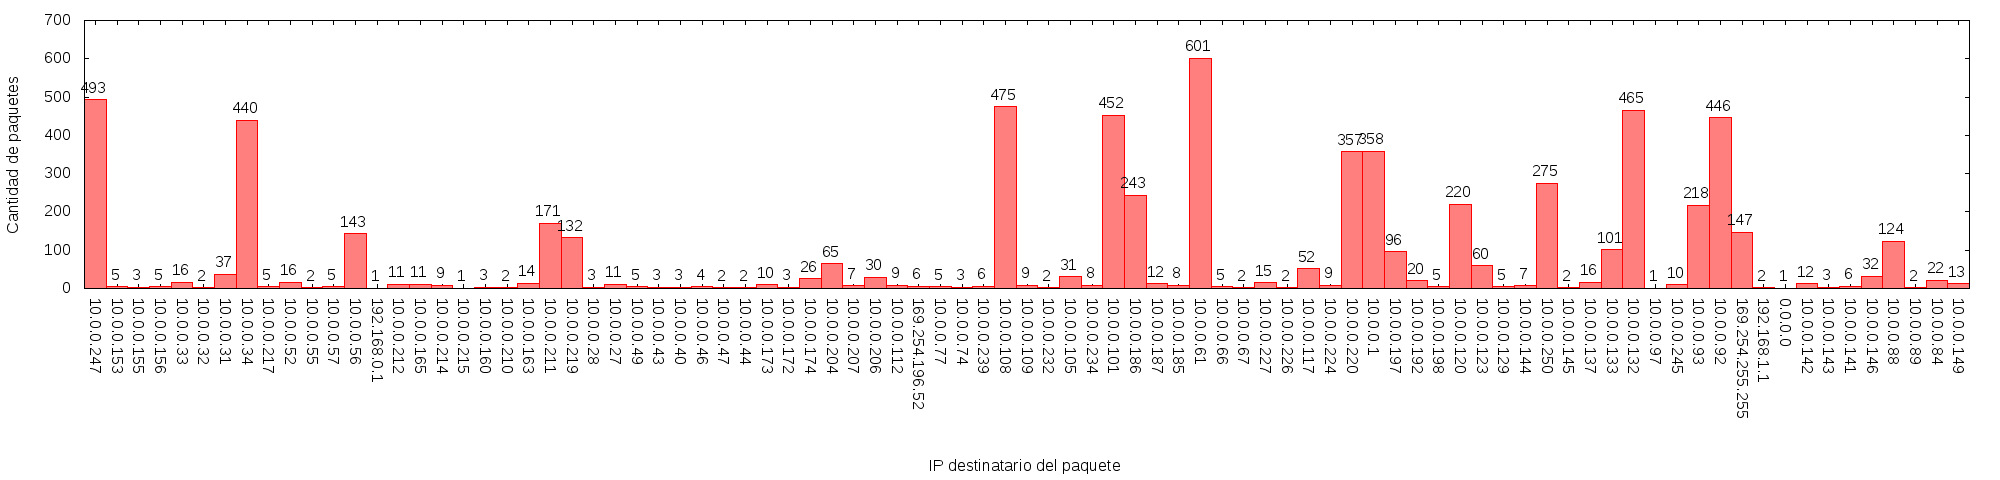
\includegraphics[width=16cm]{../mediciones/job2/dst.png}
Segunda medición
\end{center}

\begin{center}
\begin{tabular}{|c||c|c|}
\hline
 & Medición 1 & Medición 2 \\
\hline
\hline
Entropía de los protocolos & 0.792831613911 & 0.578907674515 \\
\hline
Entropía de las IPs origen de ARP & 1.53247970384 & 1.23402710535 \\
\hline
Entropía de las IPs destino de ARP & 5.53038672313 & 4.7457277713 \\
\hline
\end{tabular}
\end{center}

\subsection{Entropías}

\begin{center}
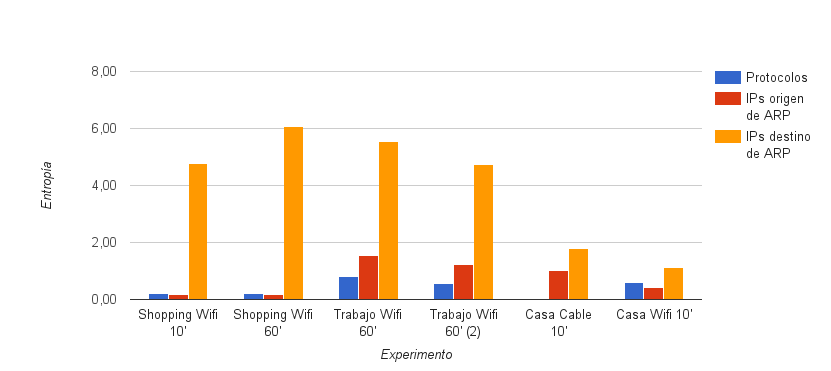
\includegraphics[width=14cm]{../mediciones/entropias.png}
\end{center}


\section{Conclusiones}
En base a los experimentos realizados, podemos concluír que ... %TODO


\newpage
\section{Apéndice}

\subsection{Enunciado}

%TODO: Agreagar enunciado

\newpage
\subsection{Figuras ampliadas}
\subsubsection{Experimento 2: Medición 60 minutos} \label{exp2_60_big}
\begin{center}
  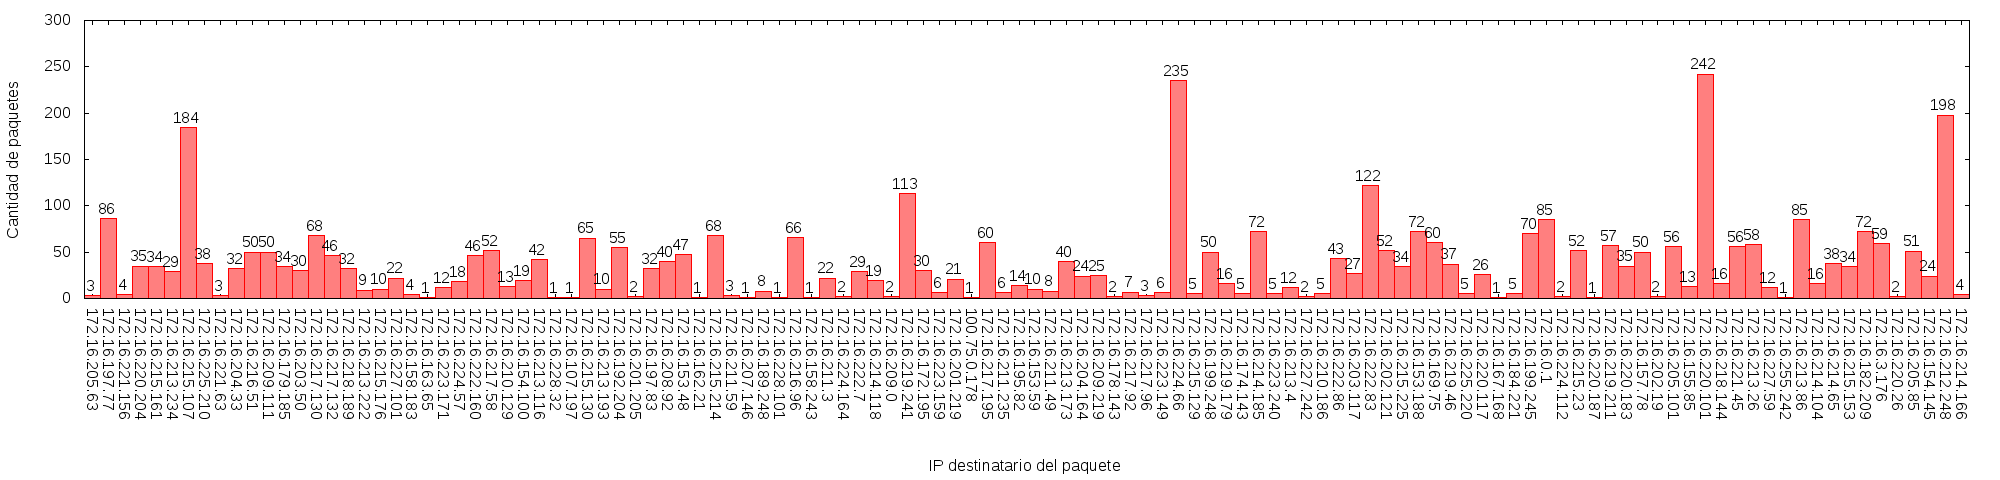
\includegraphics[angle=90, height=0.9\textheight]{../mediciones/altop-wifi-60/altop60IpsDstArp.png}
\end{center}

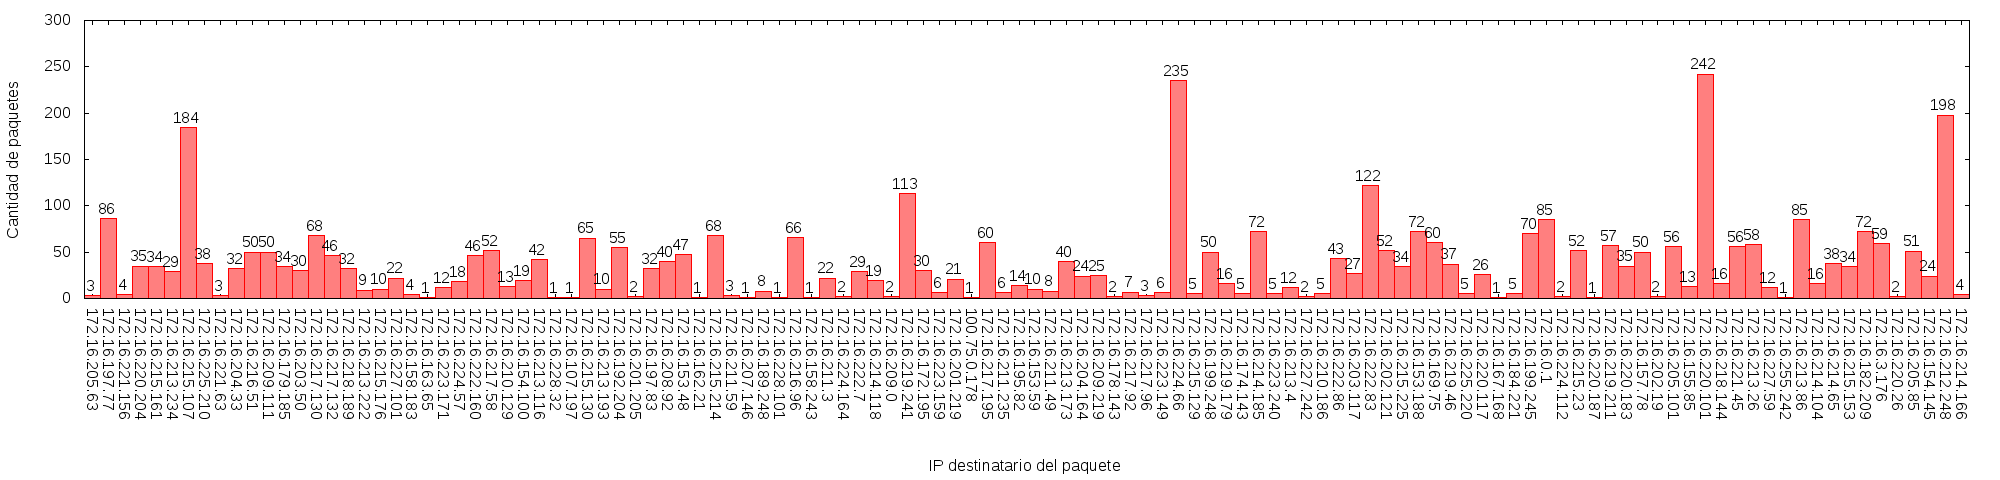
\includegraphics[width=10cm,trim={0 0 35.95cm 0},clip]{../mediciones/altop-wifi-60/altop60IpsDstArp.png}

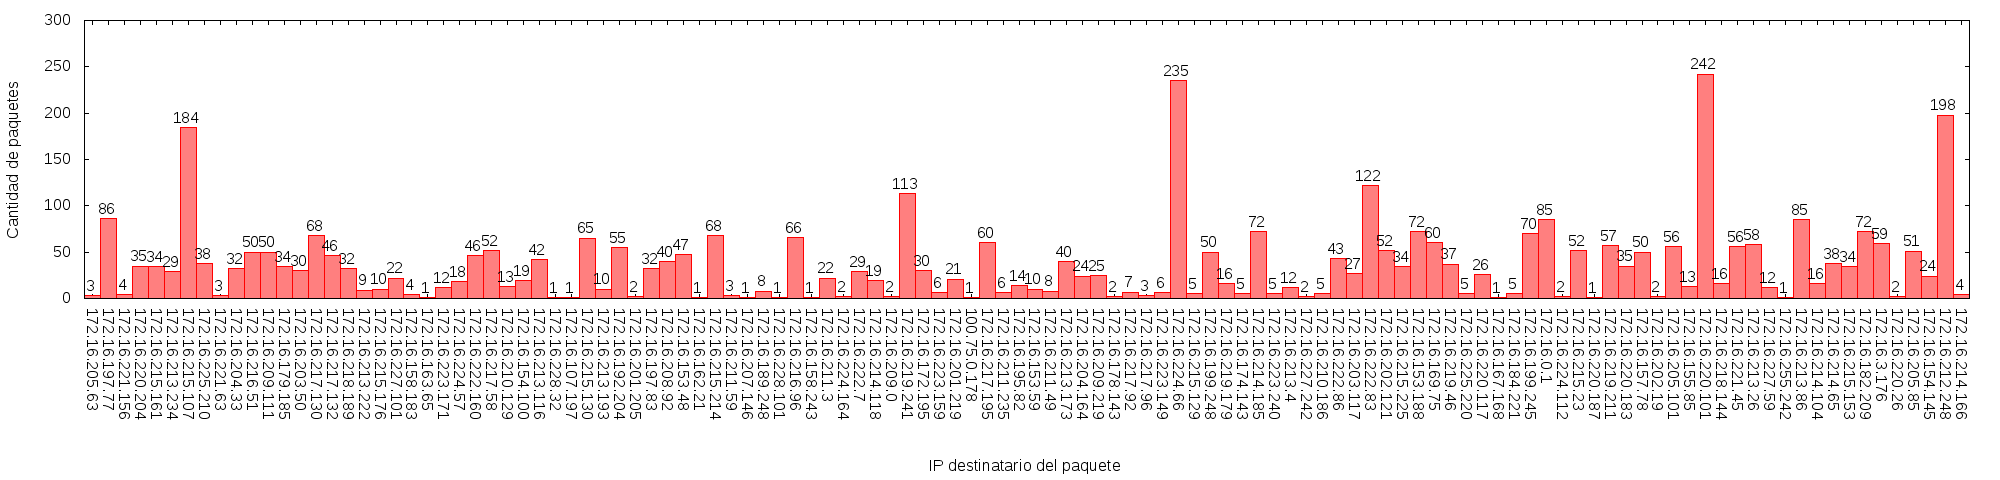
\includegraphics[width=10cm,trim={17cm 0 20.7cm 0},clip]{../mediciones/altop-wifi-60/altop60IpsDstArp.png}

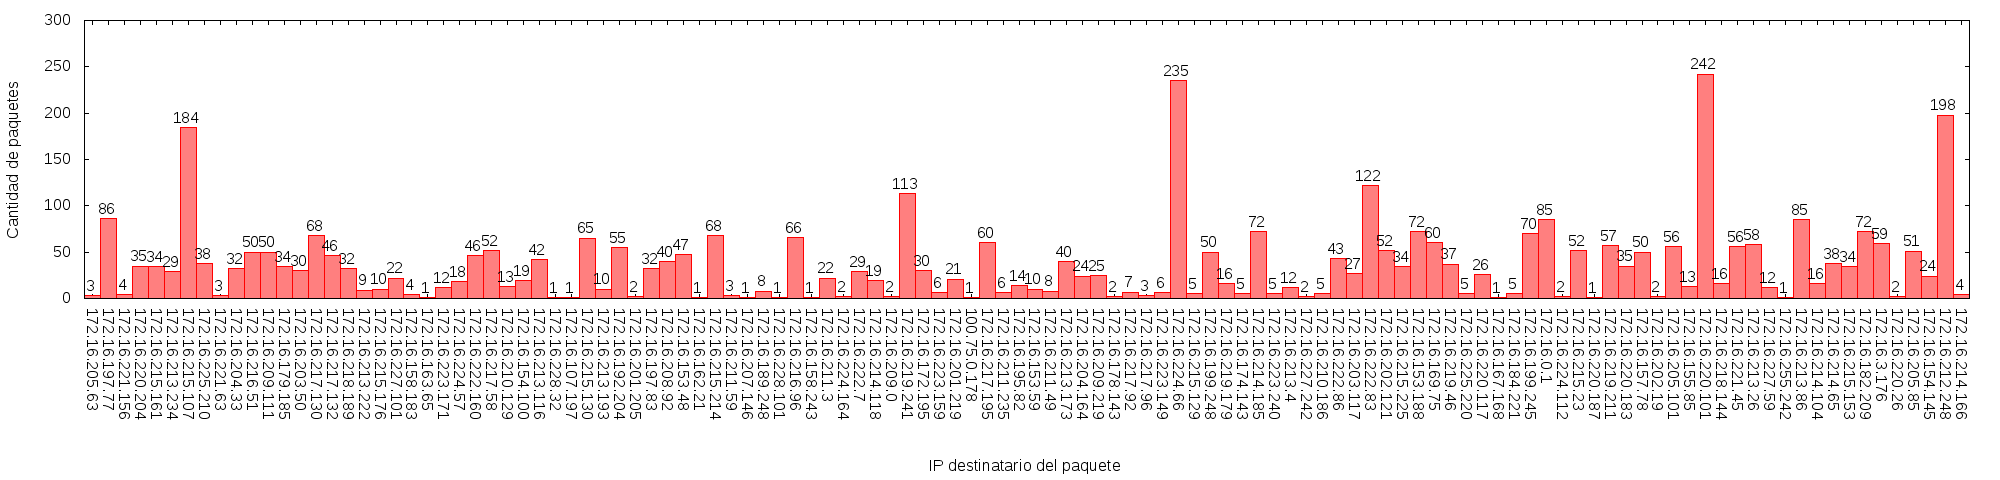
\includegraphics[width=10cm,trim={32.26cm 0 0 0},clip]{../mediciones/altop-wifi-60/altop60IpsDstArp.png}


\newpage
\bibliographystyle{plain}
\bibliography{bibliografia}

\end{document}
